As can be seen in Figure \ref{fig:CleavingFiberEnd}, a slightly darkened zone at the bottom of the fiber is observed in most of the cases. This is an unavoidable effect of the cleaving process on plastic fibers, which generates non polished end-surfaces. To remove that, a polishing process implemented by Thorlabs was applied \cite{DiamondThorlabs}. 

\textbf{Manual Polishing Method.}

The Thorlabs polishing method, shown in Figure \ref{fig:HandPolishingMethod}, consists on a kit based on a special fiber connector from Thorlabs which is used for rubbing the fibers with five different polishing papers made out of aluminum  oxyde grains, with a decreasing grain size, $30~\mu\meter$, $20~\mu\meter$, $12~\mu\meter$, $5~\mu\meter$ and $0.3~\mu\meter$, describing on the paper a shape of an 8 during 2 minuts (approximately 120 movements). 

\begin{figure}[h]
\centering
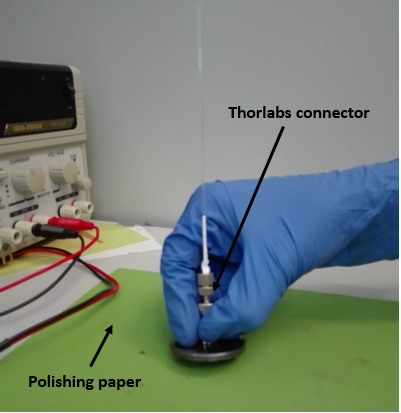
\includegraphics[scale=0.75]{4ResearchAndDevelopments/41Fibers/Hand_Polishing_Kit.png}
\caption{Manual polishing method implemented by Thorlabs.\label{fig:HandPolishingMethod}}
\end{figure}

The result obtained after polishing is shown in Figure \ref{subfig:PolishFiberEnd}, where it can be noted that the darkened zone has completely disappeared and the fiber end is uniformly transmitting light, which favors optimal coupling of the scintillating fibers to the photodetectors and transmission of scintilating photons.

\begin{figure}
\centering
    \begin{subfigure}[b]{0.5\textwidth}
    \centering
    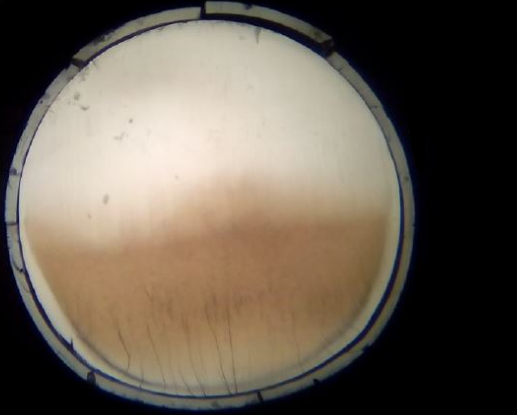
\includegraphics[width=\textwidth]{4ResearchAndDevelopments/41Fibers/CutEndFiberGood.png}  
    \caption{\label{subfig:CleaveFiberEnd}}
    \end{subfigure}
    \hfill
    \begin{subfigure}[b]{0.45\textwidth}
    \centering
    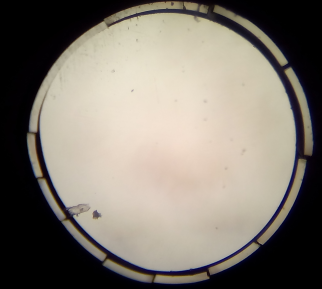
\includegraphics[width=\textwidth]{4ResearchAndDevelopments/41Fibers/CutAndPolishedFiberEnd.png}  
    \caption{\label{subfig:PolishFiberEnd}}
    \end{subfigure}
 \caption{Result of the polishing process. a) Fiber end after cleaving b) Fiber end after cleaving and hand polishing with Thorlabs technique. Pictures taken with the microscope PB 4161 from EUROMEX.}
 \label{fig:ResultofPolishingProcess}
\end{figure}

\textbf{Automatic Polishing Machine.}

The main drawback of the manual polishing method is that it takes more than 10 minutes to polish each fiber, an unaffordable time to polish thousands of fibers needed for the TRITIUM detector (see section \ref{sec:TritiumMonitor}). This is why an automated polishing process has been developed within this thesis work. The goal of this effort was to ensure a better light coupling and transmission of light of the scintillating fibers to the photosensors. 


%As mentioned above, tens of thousands of fibers had to be prepared and conditioned for the TRITIUM monitor\footnote{Tritium monitor is composed of several modules based on hundred of scintillating fibers.} (see section \ref{sec:TritiumMonitor}). Cleaving this large number of fibers with out home-made cleaving device was a relatively fast process. Polishing them however is quite time consuming, as it takes ten minutes to hand polish one fiber. Hand polishing thoudands of fibers,  would result in an unaffordable amount of time. This is why an automated polishing process has been developed within this thesis work. The goal of this effort was to ensure a better light coupling and transmission of light of the scintillating fibers to the photosensors. 

A machine was designed, built and tested in the laboratory for automatically polishing of up to one hundred plastic scintillating fibers at the same time and it is easily scalable to larger number of fibers.

\begin{figure}[h]
\centering
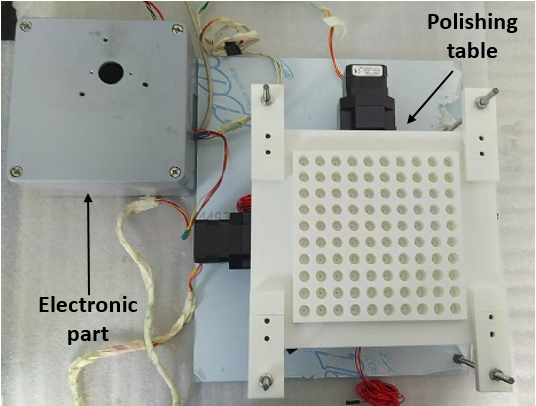
\includegraphics[scale=0.75]{4ResearchAndDevelopments/41Fibers/GeneralViewPolishingMchine.png}
\caption{Polishing machine developed for TRITIUM.\label{fig:GeneralViewPolishingMachine}}
\end{figure}
This automatic polishing machine, displayed in Figure \ref{fig:GeneralViewPolishingMachine}, consists of two main parts: 1) A polishing table, where the fibers are polished 2) The electronics, based on Arduino technology, that operates the movement of the polishing paper:

\begin{enumerate}
\item{} The polishing table, shown in Figure \ref{subfig:PolishingTable}, is composed of two parts, a static part, where the fibers are fixed, and a movable part on bottom of the previous one, where the polishing papers are fixed. It was decided to establish the polishing movement on the plate with the polishing sheets, because of its lighter weight and in order to avoid possible damaging movements to the fibers.

The static part (the fiber holder plate), shown in Figure \ref{subfig:PolishingTable}, consists of a plastic piece built with a 3D printer and locked to the system by four vertical screws. There are two nuts on each screw used to set the relative height and the inclination of fibers relative to the polishing papers. This piece contains one hundred holes in which a hundred fibers are lodged. 

As the fibers are too light ($0.16~\gram$) to make by gravity the necessary pressure on the polishing paper, a plastic belt and a piece of metal with a weight of about $1.5~\gram$ were attached to the individual fibers, as shown in Figure \ref{subfig:FiberMetailcPiece}, to increase their contact pressure, in a similar way as with the manual polishing connectors. 

The movable part of the polishing table consists of a flat PMMA plate of $18 \times 18~\cm^2$ to which the polishing paper is attached. This part is locked to structure \cite{StructureAxis} that contains two horizontal screws, perpendicular to each other, which allow its movement in the XY plane (horizontal plane), as shown in Figure \ref{subfig:HorizontalAxis}.

The polishing system contains several subminiature switches with high repeat accuracy, model DB1 6A250, mounted on a piece made with a 3D printer, shown in Figures \ref{subfig:PolishingTable}, \ref{subfig:HorizontalAxis} and \ref{subfig:3DSwitchPiece}, which are used to find the origin of coordinates when the system is reinitiated and to stop the movable part when the end of the path is reached. 

\begin{figure}
\centering
    \begin{subfigure}[b]{0.55\textwidth}
    \centering
    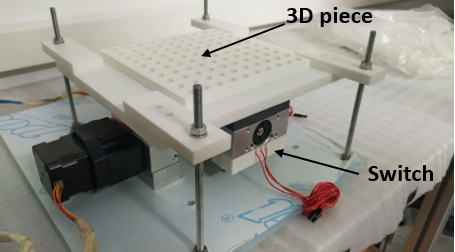
\includegraphics[width=\textwidth]{4ResearchAndDevelopments/41Fibers/PolishingTable.png}  
    \caption{\label{subfig:PolishingTable}}
    \end{subfigure}
    \hfill
    \begin{subfigure}[b]{0.3\textwidth}
    \centering
    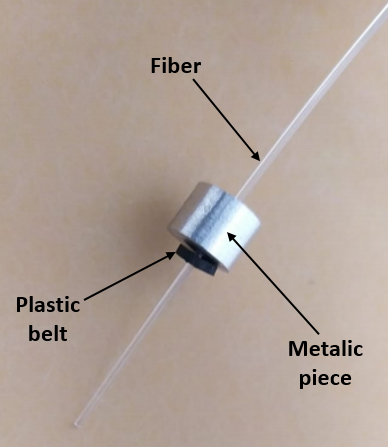
\includegraphics[width=\textwidth]{4ResearchAndDevelopments/41Fibers/PieceOfFiber.png}  
    \caption{\label{subfig:FiberMetailcPiece}}
    \end{subfigure}
    \hfill
    \begin{subfigure}[b]{0.55\textwidth}
    \centering
    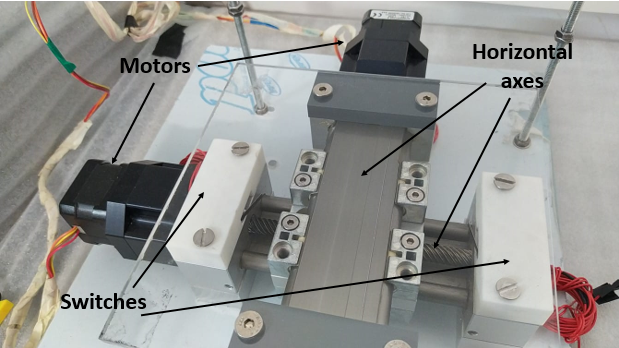
\includegraphics[width=\textwidth]{4ResearchAndDevelopments/41Fibers/HorizontalAxis2.png}  
    \caption{\label{subfig:HorizontalAxis}}
    \end{subfigure}
    \hfill
    \begin{subfigure}[b]{0.4\textwidth}
    \centering
    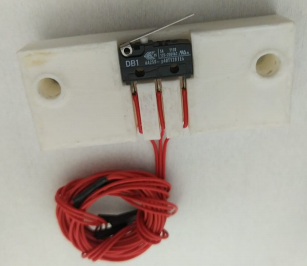
\includegraphics[width=\textwidth]{4ResearchAndDevelopments/41Fibers/Switch.png}  
    \caption{\label{subfig:3DSwitchPiece}}
    \end{subfigure}
 \caption{Components of the fiber polishing machine. a) Polishing table. b) Fiber with ballast metal piece. c) Horizontal screws and PMMA plate. d) A movement switch with its cables inserted inside its holding piece.}
 \label{fig:PolishingTable}
\end{figure}

\item{} The electronics, shown in Figure \ref{fig:ElectronicSystemPolishingMachine}, which controls the automatic movement of the polishing paper, is based on Arduino technology. It consists of two stepper motors controlled by an Arduino UNO \cite{ArduinoUNO} that uses a CNC shield \cite{CNCShield} in which two different drivers are connected to control each of this stepper motors.

%This consists of two stepper motors which move the horizontal screws on which the PMMA plate holding the polishing paper is attached

The stepper motor is a type of DC motor in which a full rotation is divided into a number of equal steps. This, it is manufactured with a number o steps per revolution, corresponding to a given stepping angle. The stepper motor used for he polishing machine are model NEMA ST4209S1404-A \cite{StepperMotors}, with bipolar voltage of $2.77~\volt_{DC}$, $1.33~\ampere$ maximum current and a stepping angle of $0.9~\degree$ ($400$ steps/rev). They can be operated with or without a position sensor for feedback control. These stepper motors are used to move the horizontal screws on which the PMMA plate that hold the polishing paper is attached.

Drivers are controllers that allow to manage stepper motors in a simple and safe way as they are used to limit the current supplied to the motors. Choosing the right controllers, with the power and the stepping mode required for the chosen stepper motors, is crucial. This is because overpowering them could rapidly be damaging, while an inadequate stepping would result in inaccurate movements of the mobile part of the polishing paper. 

Several drivers were succesively considered and tested: the most widely used driver Pololu A4988 \cite{A4988Driver} ($35~\volt$, $2~\ampere$ and $16$ steps), the driver DRV8825 ($45~\volt$, $2.5~\ampere$ and $32$ steps) and the TMC2208 \cite{TMC2208Driver} ($35~\volt$, $2.5~\ampere$ and $256$ steps) with more microstepping modes, which results in more accurate and smooth movements. This later includes a StealthChop funciton with which the driver operates in silence mode for low motor velocities. It is seen that the power provided by each stepper is enough to correctly move the stepper motors. Therefore, owing to these features, the TMC2208 driver is the one used for the control of the stepper motors since it produce the most accurate and smooth movement. The provided current to the motors is limited by the driver and the excess will be transformed into heat that has to be dissipated for the correct functioning of the drivers. 

Indeed, overheating of the drivers may cause loss of steps, producing wrong movements or even destroying the driver. Therefore, a cooling system is needed to ensure the correct operation of the polishing system. The cooling system, shown in Figure \ref{fig:ElectronicSystemPolishingMachine}, consists of a copper heat sink\footnote{The copper is one of the best thermal conductor at STP} in contact with both controllers and a fan, used to prevent heat accumulation inside the electronics box. The cooling power can be inproved by using a PELTIER cell.

\begin{figure}[h]
\centering
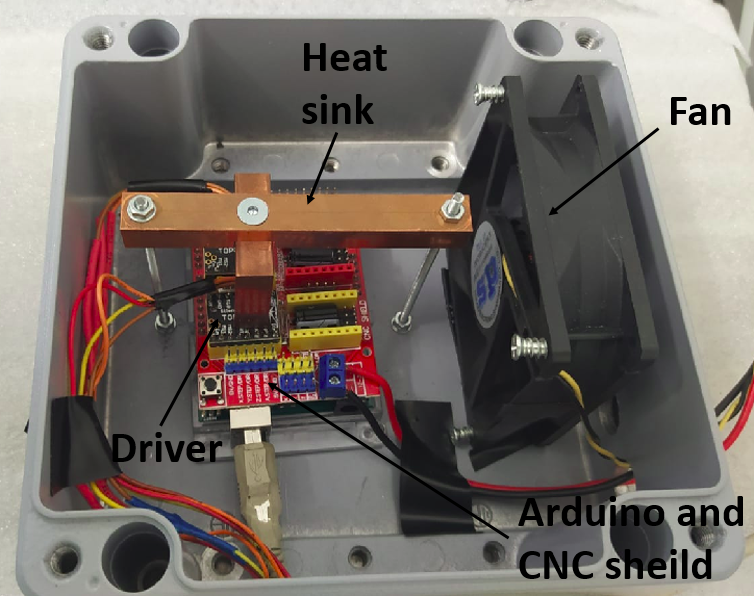
\includegraphics[scale=0.75]{4ResearchAndDevelopments/41Fibers/ElectronicPolishingMachine.png}
\caption{Electronic system of Polishing machine.\label{fig:ElectronicSystemPolishingMachine}}
\end{figure}

\end{enumerate}

Finally, this polishing machine is controlled by a Raspberry Pi computer board \cite{RaspberryPi} using the Universal G-code Sender software, a grafical interface based on the GRBL package \cite{GRBLDocumentation}. There are several usefu are loaded in this way. 
l pre-programmed functions such as "HOME" with which the system, using the switches, finds its origin of coordinate every time the system is turned on. The software also has the possibility of loading a file containing the G-code to be executed. In the fiber polishing machine, the 120 movements required for each polishing paper.

\textbf{Experimental Test.}

Finally, this machine was tested with twenty uncladded scintillating fibers of $15~\cm$ length. These fibers were arranged in a bunch and were couplet at each end to two PMTs, as shown in Figure \ref{fig:BunchWith2PMTsCoincidence}, which were read out in coincidence. The electronic scheme shown in Figure \ref{subfig:ElectronicConfiguraiton2PMT} was used to process and analyze these signals and an energy spectrum was obtained. The goal of the test was to quantify the improvement in the relative light transmission of the scintillating fibers due to the polishing process.

\begin{figure}[]
\centering
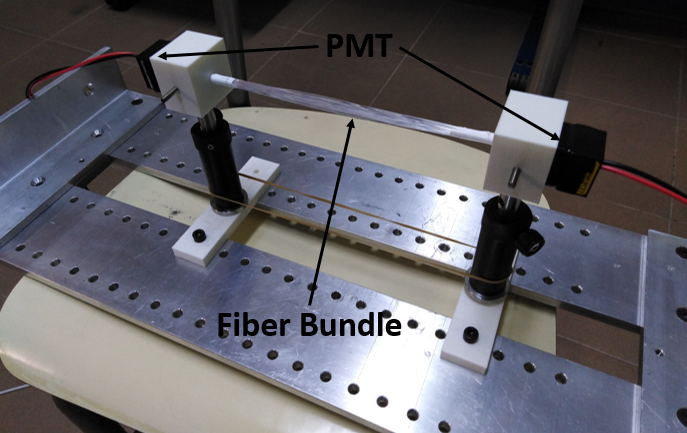
\includegraphics[scale=0.6]{4ResearchAndDevelopments/41Fibers/FiberBunch2PMTsCoincidence.png}
\caption{Setup used to test the effect of the fiber polishing on light transmission to the PMTs. This setup is placed in a dark test box for the measurements.\label{fig:BunchWith2PMTsCoincidence}}
\end{figure}

These measurements were carried out using two radioactive sources, an encapsulated $\ce{^{60}Co}$ source with gamma emissions of $1173.2~\keV$ and $1332.5~\keV$ and an activity of $715~\becquerel$, and a $\ce{^{90}Sr}$ beta source with a maximum beta energy of $545.9~\keV$ and an activity of $17.8~\kilo\becquerel$. The radioactive sources were placed next to the fiber bundle, in the middle of it (at $7.5~\cm$ from each PMT) and the energy spectra was recorded for both radioactive sources, which are shown in Figure \ref{fig:ResultsOfPolishingMachine}. This experiment was carried out inside a special light-tight box, called balck box, to ensure that the detected photons are generated by the scintillating fibers.

\begin{figure}
\centering
    \begin{subfigure}[b]{1\textwidth}
    \centering
    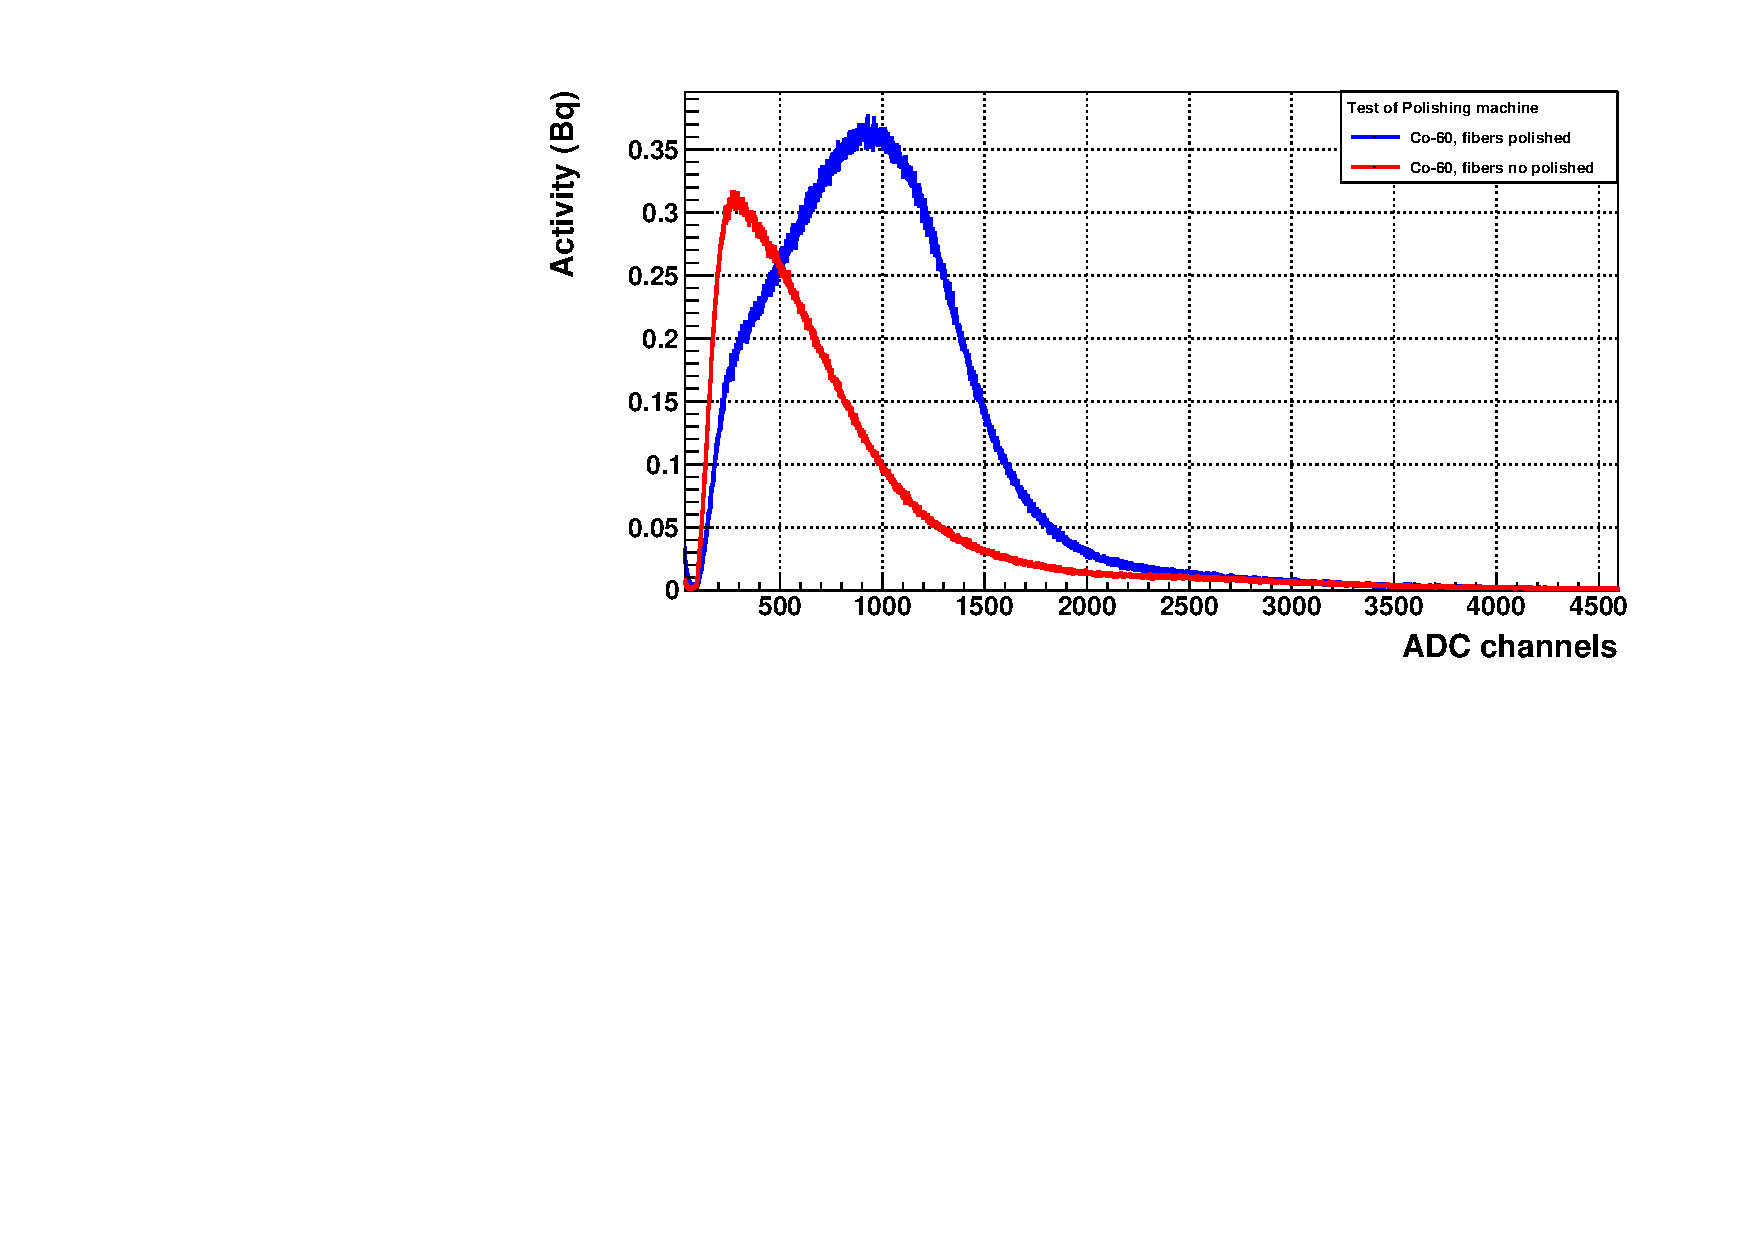
\includegraphics[width=\textwidth]{4ResearchAndDevelopments/41Fibers/Co_60_PolishingMachine_ZOOM.pdf}  
    \caption{\label{subfig:EnergySpectrumCo60PolishingTest}}
    \end{subfigure}
    \hfill
    \begin{subfigure}[b]{1\textwidth}
    \centering
    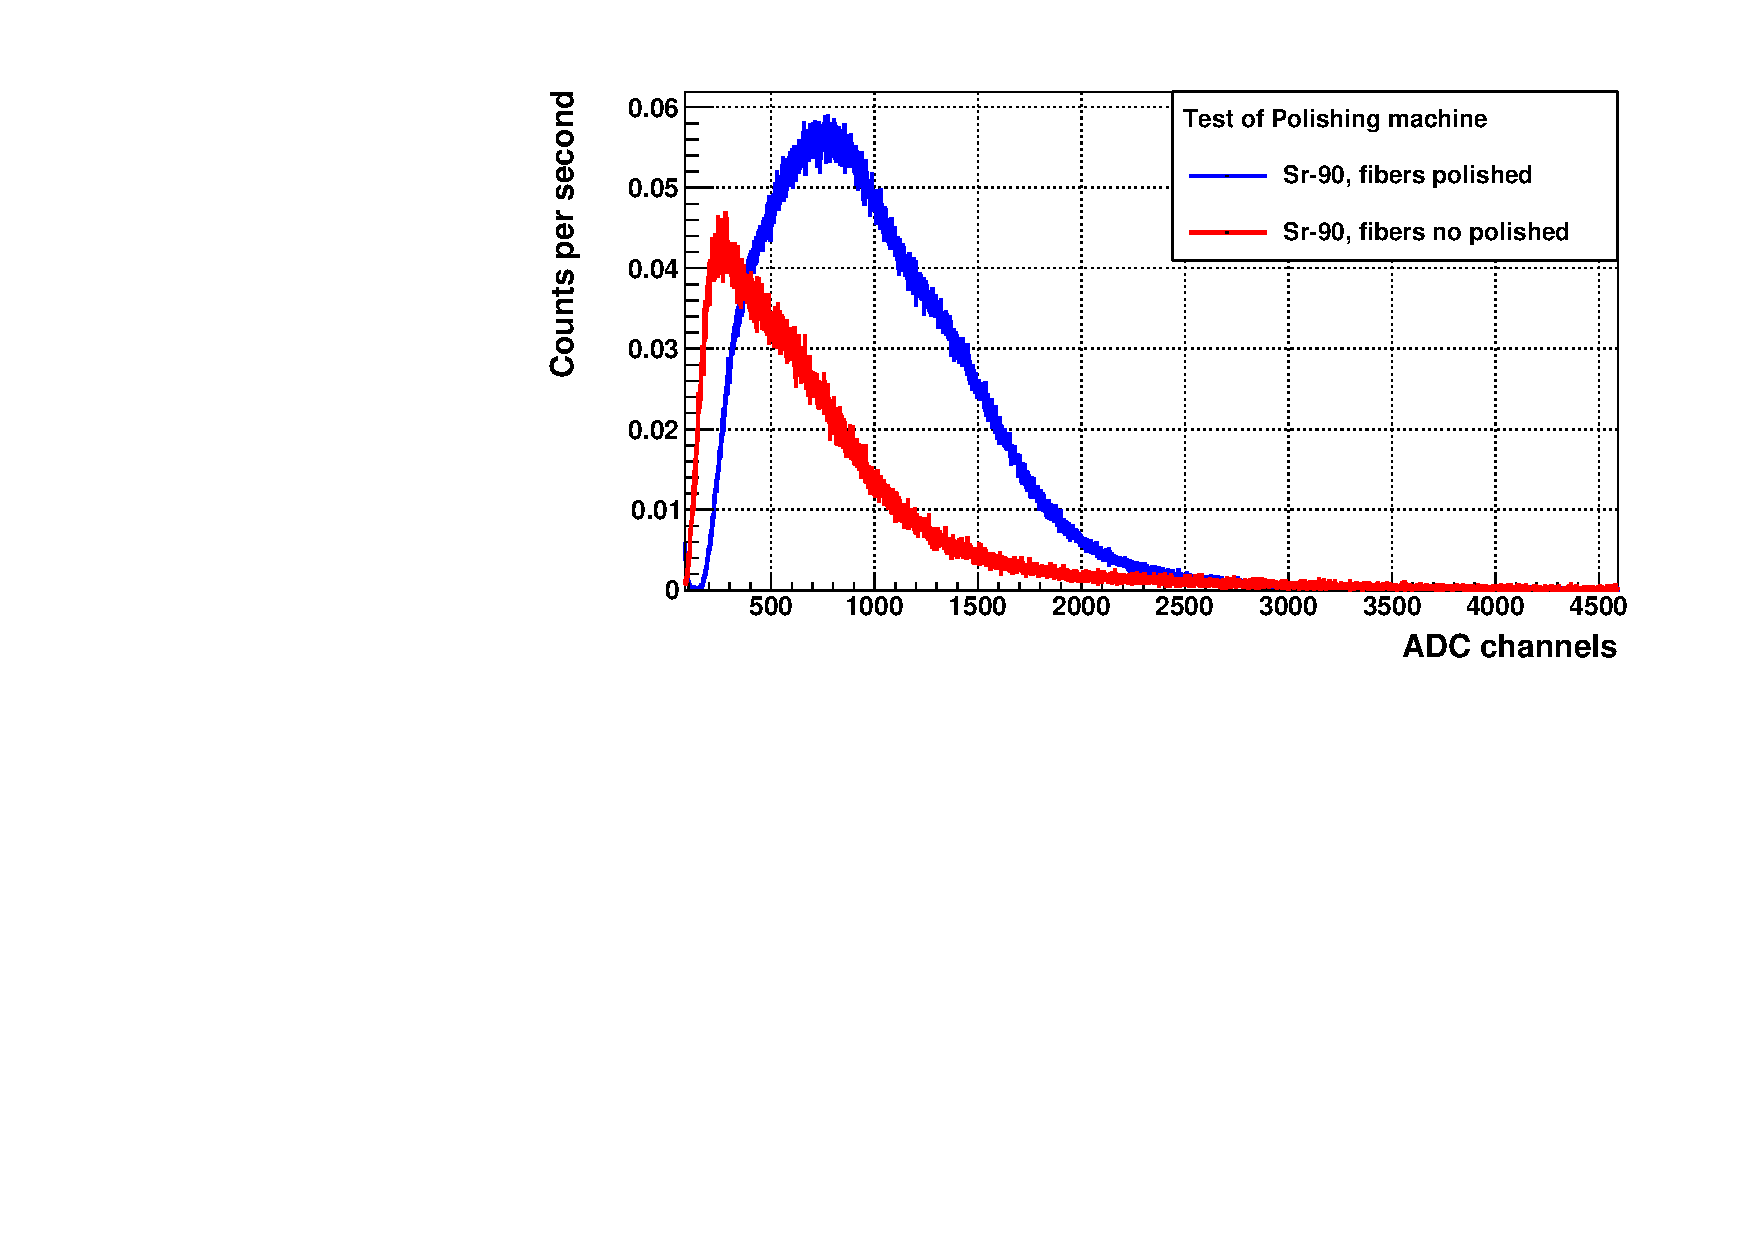
\includegraphics[width=\textwidth]{4ResearchAndDevelopments/41Fibers/Sr_90_PolishingMchine_ZOOM.pdf}  
    \caption{\label{subfig:EnergySpectrumSr90PolishingTest}}
    \end{subfigure}
 \caption{Energy spectra recorded with polished and unpolished fibers. a) for the $\ce{^{60}Co}$ source b) for the $\ce{^{90}Sr}$ source}
 \label{fig:ResultsOfPolishingMachine}
\end{figure}

As it can be seen in Figure \ref{fig:ResultsOfPolishingMachine}, both energy spectra are shifted to the right after polishing, which means that the detected events have more energy (more photons per event reach the PMTs). This improvement in photon collection was quantified by a parameter $F$ definded as,
\begin{equation}
F=\frac{A_{C}-A_{NC}}{A_{C}}
\label{eq:RelativeImprovement}
\end{equation}
where $A_{C}$ and $A_{NC}$ ae the integrals of the energy spectra measured after and before the cleaning process, respectively. It was achieved an improvement of more than 40\% ($(42 \pm 5)\%$ for gamma source and $(49 \pm 8)\%$ for beta source) with respect to the spectra before polishing. In summary, with the polishing machine, the photon collection efficiency of the fibers was improved  (mainly due to the improvement of the interface between fibers and PMTs). It is very important to achieve a high detection efficiency as the expected number of photons per tritium event is quite low, less than 20 as it has been demonstrated with simulations and experimental measurements.